\section {Introduzione}

\begin {frame}
\frametitle {Introduzione}
\begin{itemize}
	\item Le tecniche \emph{in silico} sono un'integrazione promettente alla sperimentazione \emph{in vitro}, a causa di costi elevati e potenziale scarsit\`a di informazioni preliminari
	\item I \alert{metodi formali} sono efficaci per l'analisi di sistemi complessi e permettono di ottenere informazioni quantitative, prestazionali e temporali senza errori
	\item Necessario un approccio integrato di tecniche simulative e basate su verifica perch\'e la prima presenta errori, mentre la seconda risulta spesso intrattabile
	\item <2> Caso di studio: trattamento a base di RBC ingegnerizzati per la \alert{deficienza GAMT}
	\end{itemize}

\end{frame}

\begin {frame}
\frametitle {Esempio}
\framesubtitle{Input}

\begin{columns}
	\column{.3\textwidth}
	\begin{equation*}
	E + S \xrightleftharpoons[k_{-1}]{k_1} ES \xrightarrow{k_2} E + P
	\end{equation*}
	\visible<2->{	\column{.03\textwidth}$\leadsto$
	\column{.2\textwidth}
		\begin{align*}
		r_1 &= k_1 [E][S]\\
		r_{-1} &= k_{-1}[ES]\\
		r_2 &= k_2 [ES]\\
		E &= r_1\downarrow E + r_{-1}\uparrow E + r_2 \uparrow E\\
		S &= r_1 \downarrow S + r_{-1} \uparrow S\\
		ES &= r_1 \uparrow ES + r_{-1} \downarrow ES + r_2 \downarrow ES\\
		P &= r_2 \uparrow P\\
		E &\underset{\{r_1, r_{-1}, r_2\}}\bowtie \left(S \underset{\{r_1, r_{-1}\}}\bowtie \left(ES \underset{\{r_2\}}\bowtie P\right)\right)
		\end{align*}
		
	}
	
	\visible<3->{
	\column{.03\textwidth}$\leadsto$
	\column{.25\textwidth}
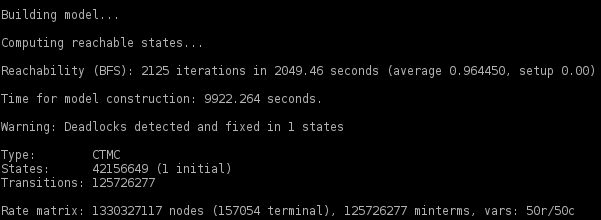
\includegraphics[width=\textwidth]{michaelis/prism.png}}
\end{columns}

\end{frame}

\begin {frame}
\frametitle {Esempio}
\framesubtitle{Output}

\begin{columns}[t]
	\column{.4\textwidth}
	\begin{block}{Simulazioni}
		\resizebox{\textwidth}{!}{
			\begin{tikzpicture}
			\begin{axis}[axis lines=middle, xmin=0, xmax=2, ymin=0, ymax=100,samples=1000, xtick={0,10,...,60}, xlabel={$t (min)$}, ylabel={$conc. (\mu M)$}, legend style={font=\tiny},
			x label style={at={(axis description cs:0.5,-0.1)},anchor=north},
			y label style={at={(axis description cs:-0.1,.5)},rotate=90,anchor=south},
			tick label style={font=\tiny},
			label style={font=\tiny},
			legend pos=outer north east,
			legend entries={$[E]$, $[S]$, $[ES]$, $[P]$},mark repeat={5}]
			
			\addplot[
			ultra thin,
			scatter,
			point meta=explicit symbolic,
			scatter/classes={
				E={mark=asterisk,draw=black,mark size=2},
				S={mark=pentagon, draw=black,mark size=2},
				ES={mark=diamond, draw=black,mark size=2},
				P={mark=o,draw=black,mark size=2}}
			]
			file{michaelis/E.txt};
			
			\addplot[
			ultra thin,
			scatter,
			point meta=explicit symbolic,
			scatter/classes={
				E={mark=asterisk,draw=black,mark size=2},
				S={mark=pentagon, draw=black,mark size=2},
				ES={mark=diamond, draw=black,mark size=2},
				P={mark=o,draw=black,mark size=2}}
			]
			file{michaelis/S.txt};
			
			\addplot[
			ultra thin,
			scatter,
			point meta=explicit symbolic,
			scatter/classes={
				E={mark=asterisk,draw=black,mark size=2},
				S={mark=pentagon, draw=black,mark size=2},
				ES={mark=diamond, draw=black,mark size=2},
				P={mark=o,draw=black,mark size=2}}
			]
			file{michaelis/ES.txt};
			
			\addplot[
			ultra thin,
			scatter,
			point meta=explicit symbolic,
			scatter/classes={
				E={mark=asterisk,draw=black,mark size=2},
				S={mark=pentagon, draw=black,mark size=2},
				ES={mark=diamond, draw=black,mark size=2},
				P={mark=o,draw=black,mark size=2}}
			]
			file{michaelis/P.txt};
			
			\end{axis}
			\end{tikzpicture}
		}
	\end{block}
	\column{.4\textwidth}
		\begin{block}{Verifiche formali}
			
			\begin{center}
			$\mathbb{P}_{=?} [\mathcal{F}^{\leq 60} [P] > 50]$
			\\\leavevmode\\\leavevmode
				``Qual \`e la probabilit\`a che la concentrazione di $P$ sia maggiore di $50 \mu M$ entro 60 minuti?''
				\\\leavevmode\\\leavevmode
				Esito: $13.1\%$ (calcolato in 134~secondi)
				\\\leavevmode
			\end{center}
		\end{block}
\end{columns}






\end{frame}

